\documentclass[14pt]{beamer}
\title[BPT:VCS:01]{Version Control System :: Session 01}
\author[TS]{TalentSprint}
\institute[L\&D]{Licensed To Skill}
\date{Version 1.0.4}
\usetheme{Madrid}

\usebackgroundtemplate{
\includegraphics[width=\paperwidth]{TS-Logo.jpg}}
%\graphicspath{{/home/tsuser/Desktop/Latex_Slides/Images/}}
\graphicspath{{../../Images/}}
%\graphicspath{{Images/} {ScreenShots/}}
\begin{document}

\begin{frame}
  \titlepage
\end{frame}

\begin{frame}{What is a Version Control System?}
  A software system that records changes to a file or set of files over time so that we can capture, track, and manage the changes to those files.
\end{frame}

\begin{frame}{Goals}
  \begin{itemize}
  \item enable people to work simultaneously, not serially.
  \item changes do not conflict with each other.
  \item archive every version.
  \end{itemize}
\end{frame}

\begin{frame}{Benefits}
  \begin{itemize}
  \item Collaboration
    \pause
  \item Change management 
    \pause
  \item Tracking evolution 
    \pause
  \item Branching
  \end{itemize}
\end{frame}

\begin{frame}{Common terms}
  \begin{itemize}
  \item Repository 
    \pause
  \item Working copy 
    \pause
  \item Trunk 
    \pause
  \item Revision
  \end{itemize}
\end{frame}

\begin{frame}{Common Operations}
  \begin{itemize}
  \item Checkout
    \pause
  \item Commit 
    \pause
  \item Update
    \pause
  \item Revert 
  \end{itemize}
\end{frame}

\begin{frame}{Types of VCS }
  \begin{itemize}
  \item Local Version Control Systems
    \begin{itemize}
    \item SCCS (1972), RCS (1982)
    \end{itemize}
    \pause
  \item Centralized Version Control Systems
    \begin{itemize}
    \item CVS (1986), SVN (2000)
    \end{itemize}
    \pause
  \item Distributed Version Control Systems
    \begin{itemize}
    \item DCVS (2002), Git (2005), Mercurial (2005) 
    \end{itemize}
  \end{itemize}
\end{frame}

\begin{frame}{Local Version Control System}
  \begin{center}
    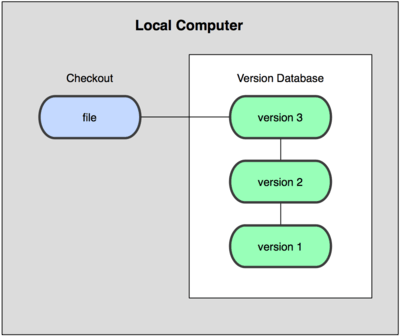
\includegraphics[scale=0.5]{LocalVCS.png}
  \end{center}
\end{frame}

\begin{frame}{Centralized Version Control System}
  \begin{center}
    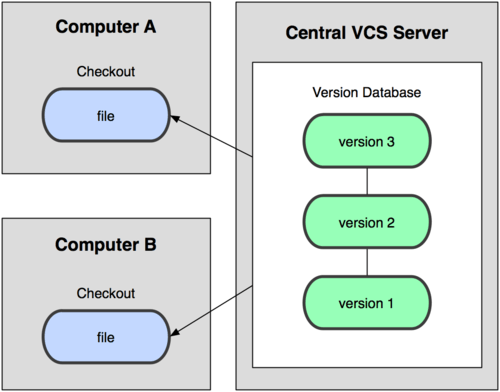
\includegraphics[scale=0.45]{CentralizedVCS.png}
  \end{center}
\end{frame}

\begin{frame}{Distributed Version Control System}
  \begin{center}
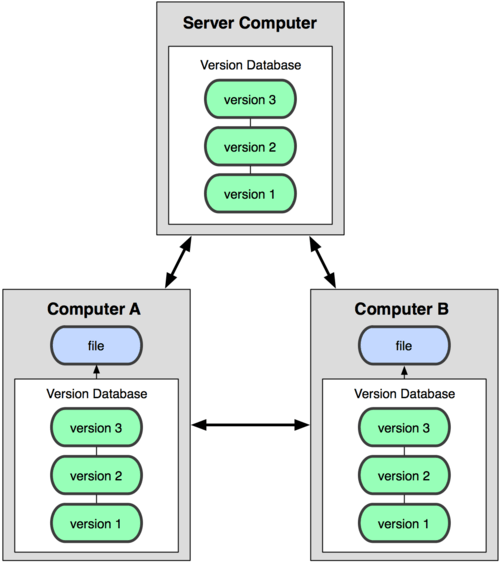
\includegraphics[scale=0.38]{DistributedVCS.png}
  \end{center}
\end{frame}

\end{document}
